
Island biogeography theory has been widely applied to predict properties of species assemblages across islands, but its relevance for species interaction networks remains less clear. Here, we take a macroecological approach to investigate how bipartite interaction networks between free-living hosts and helminth parasites vary across gradients of island area and isolation. Using the current largest published global collection of host-helminth interaction records, we tested the relationship between island characteristics and host richness, helminth richness, and interaction nestedness. We found that host and helminth richness were positively associated with island area and mainland connectivity as measured by surrounding landmass proportion, though unrelated to distance to the nearest mainland. In contrast, nestedness showed only a weak positive relationship with island area and was unrelated to mainland connectivity. These results suggest that island characteristics shape the size of host-parasite assemblages more predictably than the organization of interactions within them. Our findings extend island biogeographic perspectives to antagonistic interaction networks and motivate future work examining how host-mediated colonization and parasite specialization contribute to the assembly of antagonistic network structure across space.



\clearpage
%-----------------------------

%\subsubsection*{Island biogeography and how it blends well with current macroecological ideas}
\section*{\textbf{\underline{Abstract}}}
Island biogeography theory posits that island area and distance to the mainland combine to constrain species richness on islands through effects on extinction and colonization, respectively \citep{macarthur2001}. Despite being developed well over fifty years ago, it maintains an active research area, with numerous open questions \citep{patino2017}. This is perhaps a result of the ways that island biogeography theory can be used to inform other ecological relationships. For instance, island biogeography theory is quite closely linked to the examination of species-area relationships \citep{losos2000, peay2007}. Further, island biogeography theory is a simple base on which to build, as seen by extensions to species functional trait variation \citep{jacquet2017}, predator-prey interactions \citep{gravel2011}, and compositional differences between communities \citep{lu2018}. It is clear that island biogeography theory has the potential to inform trophic and community scale phenomena. 
\end{Abstract}


\subsection*{Introduction}
%\subsubsection*{Island biogeog and species interaction networks}
\paragraph*{}
The increasing availability of ecological data has encouraged the study of large-scale processes such as island biogeography theory. This data availability has also promoted the study of species interaction networks \citep{delmas2019, dormann2017}, which characterize the interactions between two (or more) trophic groups (e.g., plant species and their pollinators). This has permitted examinations into how spatial and environmental gradients influence the structure of these species interaction networks \citep{tylianakis2017}, with structure defined using measures such as nestedness and modularity \citep{dalsgaard2013, dormann2017}, which capture the tendency of species interactions to form proper subsets of species with more interactions (nestedness) or cliques of interacting species (modularity). Regardless of the measure used to capture aspects of species interactions, there is mounting evidence that species interactions follow the same patterns as species richness with regards to island area and isolation \citep{sugiura2010, dormann2017, tylianakis2017}. For instance, \citet{traveset2016} compared mainland and island plant-pollinator networks, finding that isolated oceanic islands had the lowest species richness -- in agreement with predictions from classic island biogeography theory -- and the lowest interaction diversity and highest plant niche overlap. That is, as the richness of plants and pollinators decreased with isolation, so did the structure of the interactions between plant and pollinator species. Relatedly, \citet{dalsgaard2013} found that species interaction networks tended to be modular on islands, further linking island biogeography with the study of species interaction networks. But how do we interpret the effects of island isolation and area on species interactions?




%\subsubsection*{How is the original theory related to network structure?}
\paragraph*{}
Classical biogeography studies posit that the species richness of oceanic islands is largely determined by the equilibrium between species colonization and extinction rates. Islands closer to mainland sources are colonized by new species at a higher rate, while islands with larger areas exhibit lower extinction rates. However, the interpretation of the influence of island isolation and area on the structure of species interaction networks must be different. That is, the richness of interacting species, even if driven by a balance between colonization and extinction rates, should not necessarily influence the overall structure of species interactions. For instance, if species interactions are conserved between mainland and island populations -- as evidenced by \citet{carstensen2018} -- then differences between mainland and island species interaction networks should be minimal. However, there are other reasons why island area could influence network structure. Larger islands tend to have more diverse habitat types than smaller islands, and species habitat preferences can contribute to modularity of interaction networks by reducing niche overlap between groups of habitat specialists \citep{santos2016}. Meanwhile, island isolation, as noted above, is likely unrelated to network structure, provided that species interactions are not overly plastic (i.e., species cannot readily change the set of species they interact with), or that species dispersal ability is directly related to specialization (i.e., good dispersers interact with many species).






%\subsubsection*{Thesis}
\paragraph*{}
It may be infeasible to provide tests of the underlying mechanisms which drive relationships between island isolation or area and properties of species interaction networks. However, demonstrations of the existence of the scaling relationships themselves are useful in identifying groups of species or types of interactions which modify the strength or directionality of effect of island characteristics on species interactions. For instance, while studies examining mutualistic network structure across islands are becoming increasingly common \citep{traveset2016, dalsgaard2013, sugiura2010, trojelsgaard2013}, comparable studies of antagonistic networks have lagged behind (but see \citep{gravel2011}). However, antagonistic and mutualistic networks often have quite different structural properties, potentially owing to the intrinsic difference in the effect of the species interaction (i.e., the cost of parasitism and the benefits of mutualism). Here, we examine the relationship between host-parasite network structure and island isolation and size, using host-helminth interaction data from 61 islands. First, we examined the relationship between species richness and island isolation and size, in accordance with traditional island biogeography theory. Second, we examined how a key measure of ecological network structure, interaction nestedness, scales with island characteristics. Overall, our findings suggest that while the diversity of host-parasite assemblages varies predictably with island characteristics, the structure of their interaction networks shows a more limited association. Reconciling the differences between mutualistic and antagonistic network structures among islands may provide insight into how island isolation and area are mechanistically related to species interactions and network structure.














%----------
\section*{Methods}

\subsubsection*{Host - helminth interaction data}
Records of helminth parasite occurrence on host species were obtained from the parasite database of the London Natural History Museum (LNHM) \citep{gibson2005}, and accessed programmatically using the \texttt{helminthR} package \citep{helminthr}. These data currently represent one of the largest sources of host-parasite interaction data \citep{dallas2018}, despite being restricted to helminth parasites, including Platyhelminthes (trematodes and cestodes), Acanthocephalans, and Nematodes \citep{gibson2005}. We started by identifying a total of 62 islands for which host-helminth interaction data were recorded (Figure \ref{fig:concept}). After filtering out host and helminth species not identified to the species level, this comprised a total of 7294 host-helminth species pairs across 2651 helminth species and 1980 host species.


\subsubsection*{Island isolation and size measurement}
Data characterizing the geography of islands were retrieved from \citep{Weigelt2013}, including island area (km$^2$). We measure island isolation through distance to the nearest mainland (km), and surrounding landmass proportion (SLMP), calculated as the proportion of land area within 100, 1000, and 10,000 km buffers. This metric accounts for both spatial variation in mainland connection as well as nearby island connections, and has been shown to be more robust than distance per se in explaining insular plant diversity \citep{weigelt2013quantifying}. To roughly account for historical connectivity, we also extract whether or not an island had terrestrial connections to the mainland during the last glacial maximum (GMMC). Records within the LNHM dataset were georeferenced to an island chain or series (e.g. Trinidad \& Tobago) were assigned to the largest island within the group (e.g. Trinidad). Data from \citep{Weigelt2013} were available for all but one island in our data (South Shetlands), an Antarctic island with only seabird and pinniped infection records, which we excluded from our analysis. 


\subsubsection*{Quantifying host-helminth network structure}

We related island characteristics to both species richness estimates and to measures of interaction network structure. Measures of species richness for both hosts and helminths were obtained from the London Natural History Museum data, as described above. To quantify network structure, we estimated interaction nestedness, a commonly measured aspect of network structure found to be related to network structural stability \citep{thebault2010stability, dallas2015co, valdovinos2019mutualistic} and resilience \citep{thebault2010stability, suweis2013emergence}. However, some measures of nestedness may be related to network size (number of interacting species)\citep{bascompte2003nested, nielsen2007ecological}, which creates an odd circularity where a significant effect of island area or isolation on species richness would automatically manifest in an effect on network structure. 


One method for addressing the difficulty in comparing network structure measures between networks is to measure the difference between the empirical statistic and a distribution of the statistic obtained from null model randomization. This procedure has recently been criticized as not removing the effects of network size \citep{chagnon2015}, specifically for nestedness \citep{strona2014, song2017some}. Instead, we opted to use $NODF_c$, a normalized version of the classic nestedness metric based on overlap and decreasing fill proposed by \citet{song2017some}. Calculated as $NODF_c = NODF_n/(C\cdot \log(S))$, where $NODF_n$ represents the relative observed connectance of a given graph given its maximum possible value ($NODF/max(NODF)$), and $C$ and $S$ represent the connectance and the geometric mean of the number of nodes of each class, respectively. \citet{song2017some} show that this normalized metric is insensitive to network size, and thus appropriate for comparing network structure across biogeographic scales. Computation of the $NODF_c$ was performed using a hill-climbing algorithm as implemented in the $maxNODF$ package \citep{hoeppke2021maxnodf}. For some networks with a small number of interacting species, the set of possible network configurations is too small to make meaningful inference; as such we excluded islands with five or less species within their networks ($n$ = 12). Across the remaining 47 islands, most contained networks with multiple disconnected components (modules of species with no direct linkages that connected them, $n$ = 35). As NODF is not directly measurable in disconnected networks, for networks containing multiple connected components we added the minimum number of links necessary to create a single component when calculating the maximum potential NODF value \citep{hoeppke2021maxnodf}. We demonstrate in the Supplemental Materials how the use of network structure measures that contain the influence of network size would lead to incorrect conclusions regarding the influence of island area and isolation on network structure. 

\paragraph*{Statistical Analysis}
Relationships between species richness and island characteristics were modeled as multivariate negative binomial regressions as implemented in the MASS package \citep{MASS2002}. We utilized negative binomial regressions as both Poisson and Quasi-poisson regression models exhibited significant overdispersion (see Supplemental Materials). As our alternative metrics of isolation (log distance to mainland and SLMP) were significantly negatively correlated ($\rho$ = -0.768, $p$ = 1.94e-12), we did not include both in the same model and instead used AIC to compare across metrics. The impact of island characteristics on the $NODF_c$ was modeled as a multivariate linear model using a Gaussian error distribution and logit link. Model fits were inspected through analysis of deviance and visual inspection of standard model diagnostic visualizations. Models of the effect on historical mainland connectivity (GMCC) on diversity and network characteristics were fit separately under the same framework as described above, as well as through a Wilcoxon signed-rank test. 


%-----------------------------
\section*{Results}

\subsubsection*{Species richness and island characteristics}
Island biogeography theory predicts that species richness will be negatively related to distance from a mainland (as a result of low dispersal success to distant islands), and positively related to island area (larger islands support more "stable" populations). We find evidence for an influence of area on species richness of both hosts ($\beta = $ 0.419, $p =$ 2.43e-12) and helminths ($\beta =$ 0.391, $p <$ 1.42e-10). Interestingly, host and helminth richness increased at nearly the same rate with island area. In contrast to the influence of island area, we failed to detect any influence of distance to the mainland on host ($\rho = $ -0.189, $p =$ 0.182) or helminth ($\beta = $  -0.221, $p =$ 0.116) species richness (Figure \ref{fig:islandBG}). However, when accounting for island connectivity through SLMP, we detected a positive relationship between surrounding land area and richness of both hosts ($\beta=$1.54, $p=$0.00161) and helminths ($\beta=$1.74, $p=$0.000262). 


\subsubsection*{Network structure and island characteristics}

Many measures of nestedness are sensitive to the effects of network size. In this case, network size is the species richness of host and parasite species in the network, which we found to be related to island area and SLMP (but not distance to the mainland; Figure \ref{fig:islandBG}). Using a nestedness measure that is related to network size would therefore lead to the conclusion that network structure follows a similar gradient as species richness (see Supplemental Material). Here, we use a measure of nestedness that is insensitive to network size, $NODF_c$. Using this measure, we detect a positive relationship between island area and interaction nestedness; larger islands have more nested host-helminth networks ($\beta$=0.325, $p=$0.0473, Figure \ref{fig:networkBG}). We failed to detect any relationship between network nestedness and maximum elevation, distance to mainland, or SLMP. 


% TAD: check results for tense issues. I've fixed a bunch of switches from past to present tense above, but I might have missed one or two. 




%Lastly, there was no clear spatial gradient in nestedness, suggesting that latitude or spatially-autocorrelated environmental variation are unlikely to drive network structure (Figure \ref{fig:nestMap}). This supports previous findings that antagonistic networks tend to be structured independently of latitude \citep{morris2014}.

%Grant Q: Do we still want to include this? I like it, but I don't know if that + the GMMC stuff is too many figures. 

\subsection*{Prehistoric Connectivity}

Independent of contemporary island area or distance to mainland, historical landbridge connections may alter species assemblages or network characteristics by influencing dispersal processes. We found that islands that had terrestrial mainland connections during the last glacial maximum tended to have higher host ($\beta=$1.61, $p=$9.58e-05) and helminth diversity ($\beta=$1.59, $p=8.11e-05$, Figure \ref{fig:GMMC}). Despite differences in richness, interaction networks did not differ in nestedness across GMMC status ($p=$0.71).  




%-----------------------------
\section*{Discussion}

\paragraph*{} Overall, the relationships we observed between island characteristics and the species richness of both hosts and helminth parasites are broadly consistent with predictions from classical island biogeography theory for free-living species, but nestedness showed a more limited pattern, responding weakly to island area and not to either measure of island connectivity. This suggests that island characteristics shape the size of host-parasite assemblages more predictably than they shape the organization of interactions within those assemblages. The framework of island biogeography predicts higher species richness on larger islands, in part because larger areas can support larger populations and thus lower extinction rates \citep{macarthur2001}, as well as greater habitat heterogeneity that accommodates a wider diversity of species \citep{triantis2008measurements, hortal2009island, macdonald2018theory}. Consistent with these expectations, we find a significant positive correlation between island area and the species richness of both hosts and helminths \ref{fig:islandBG}. 

\paragraph*{} Classical theory also predicts reduced diversity on islands that are more isolated from mainland source pools due to lower colonization rates \citep{macarthur2001}. While we do not detect a direct effect of distance to the mainland on species richness, we do observe a significant positive relationship between species richness and island connectivity, as measured by surrounding landmass proportion (SLMP), for both hosts and helminth parasites. Although distance and connectivity are related metrics, SLMP incorporates both proximity and the size and configuration of surrounding landmasses (including large neighboring islands), and may therefore provide a more accurate proxy for colonization potential \citep{Weigelt2013, weigelt2013quantifying, barreto2021area}. 

\paragraph*{} Species interaction networks on larger islands tend to be more nested than those on smaller islands \ref{fig:networkBG}, but this effect was generally weak ($R^2 = $0.086). In diverse communities, patterns of asymmetric specialization (i.e., specialist parasites tend to interact with hosts with high parasite richness, while the parasite communities of hosts with few associated parasites are dominated by generalist species) results in interaction nestedness \citep{vazquez2005species, lima2012patterns}. Significant interaction nestedness has been observed in a number of parasitic systems \citep{krasnov2011nestedness, lima2012patterns, guerra2016host}, and island host-helminth networks may be smaller subsets of more regionally nested source networks. If so, larger islands may more closely reflect the structural properties of these regional pools, while the comparatively depauperate networks of smaller islands may not fully preserve this nested architecture. Alternatively, the relationship between island area and nestedness may reflect non-random assembly if colonization or extinction probabilities are associated with host or parasite specialization. For example, parasites with broad host ranges, high prevalence, or those associated with abundant or highly mobile hosts may be more likely to colonize and persist on islands, while specialist parasites may be disproportionately absent from smaller islands.  

\paragraph*{} While some attention has been paid to the island biogeography of mutualistic networks \citep{sugiura2010, dalsgaard2013, traveset2016, nogales2024review}, the processes underpinning them are fundamentally different. Among these is the role of co-colonization. In many mutualistic networks, potential interaction partners may disperse and establish on islands relatively independently. In contrast, helminths generally have much lower dispersal capacity than their free-living hosts \citep{poulin2004macroecological}. As such, the dispersal of parasites to new islands is largely dependent on patterns of host dispersal \citep{font2003global, bataille2017colonization}. Parasites that have high prevalence of infection or broad host ranges may be more likely to colonize new islands. For example, parasites with sufficiently broad ranges may be able to disperse to new areas via transient hosts, even if those species do not establish persistent populations on a given island (\citet{ellis2023host} give an example with avian malaria). Alternatively, specialist species with close host associations may be more likely to be retained during colonizations \citep{schatz2023patterns}. Thus, generalist parasites may have more opportunities to colonize new islands, while some specialists may be more likely to persist when their hosts successfully establish, making the relationship between specialization and colonization potential non-linear. These linkages between host range and colonization potential may induce a biotic filter that ultimately affects network structural properties. Understanding how parasite colonization dynamics scale up to affect resulting species interaction networks across gradients is an outstanding question. 

\paragraph*{} The mechanisms underlying island-area effects on host-helminth network structure remain difficult to resolve in part because parasite occurrence and interaction data may be shaped by both biological features and sampling limitations \citep{nielsen2007ecological, llopis2023sensitivity}. The sampling of parasite communities is inherently difficult, and is limited by the availability of survey effort and taxonomic expertise. Additionally, for many helminth taxa, we have incomplete information about which hosts they are capable of infecting in nature, making it difficult to determine whether unobserved interactions represent true absences or merely incomplete sampling \citep{poulin2016missing, walker2017uncertain, farrell2022predicting}. As a result, the networks analyzed here are unlikely to represent complete characterizations of island host-helminth communities, especially on very small islands with limited sampling effort or very large islands with highly diverse host and parasite faunas. More complete and effort-standardized surveys of host and parasite communities, paired with better characterization of helminth host ranges through surveillance and experimental infection studies, may help clarify the mechanisms determining parasite colonization, persistence, and network structure across biogeographical gradients.

\paragraph*{} However, in their current form, large-data repositories like the London Natural History Museum \citet{gibson2005} still provide the opportunity to investigate the structure of parasitic communities at macroecological scales, and can motivate these further data collection efforts. To our knowledge, ours is the first study to examine the structural properties of host-parasite networks in an island biogeography context. The increasing availability of open species interaction data spanning wide geographic, taxonomic, and temporal scales provides new opportunities to better understand large-scale determinants of network structural properties and their consequences for community assembly. By looking across geographic and environmental gradients, we show that island characteristics may shape the size of host-parasite assemblages more predictably than the organization of interactions within them, while also highlighting the need to understand how host-mediated colonization shapes antagonistic network structure across environments.

\clearpage 
\bibliographystyle{plainnat} 
\bibliography{var} 
\clearpage


\section*{Figures}


\begin{figure}[h!]
  \begin{center}
    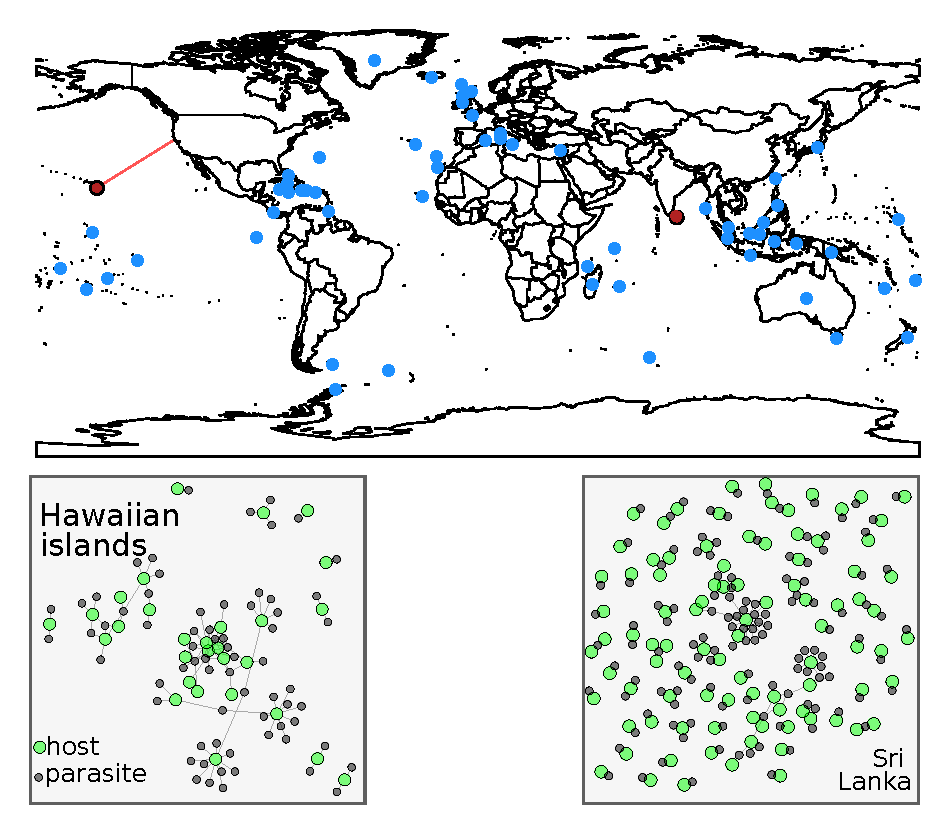
\includegraphics[width=\textwidth]{HelmBiogeog/Figures/conceptual/concept.pdf}
    \caption{Both distance to mainland and island area may influence species richness and host-helminth network structure. Islands considered in the analysis are in blue, with two example networks from the Hawaiian islands and Sri Lanka highlighted in red. Hawaii is much smaller and more distant to the mainland, and also has lower species richness relative to Sri Lanka. }
    \label{fig:concept}
  \end{center}
\end{figure}

\clearpage


\begin{figure}[h!]
  \centering
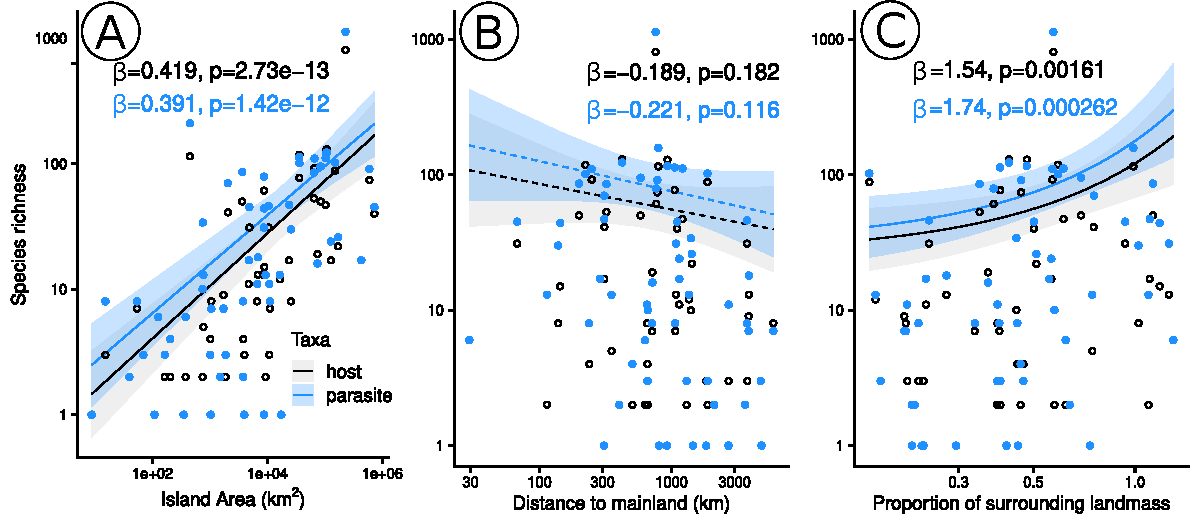
\includegraphics[width=\linewidth]{HelmBiogeog/Figures/NB_MarginalPlots_Wide.pdf}
  \caption{Traditional island biogeography theory relates species richness to the distance to the mainland (i.e., isolation) and island area. We detect a significant positive effect of island area on both helminth parasite and host richness (A), but found no significant effect of isolation as measured by distance to mainland (B). When measuring island isolation through surrounding landmass proportion, we did detect a weak but significant positive effect of island connectivity on both helminth and host richness (C). Plotted lines represent fitted relationships from a negative binomial multivariate regression model, assuming mean values of non-focal predictor variables. Significant relationships represented as solid lines; shaded regions represent 95\% confidence intervals.}
  \label{fig:islandBG}
\end{figure}

\clearpage

\begin{figure}[h!]
  \begin{center}
    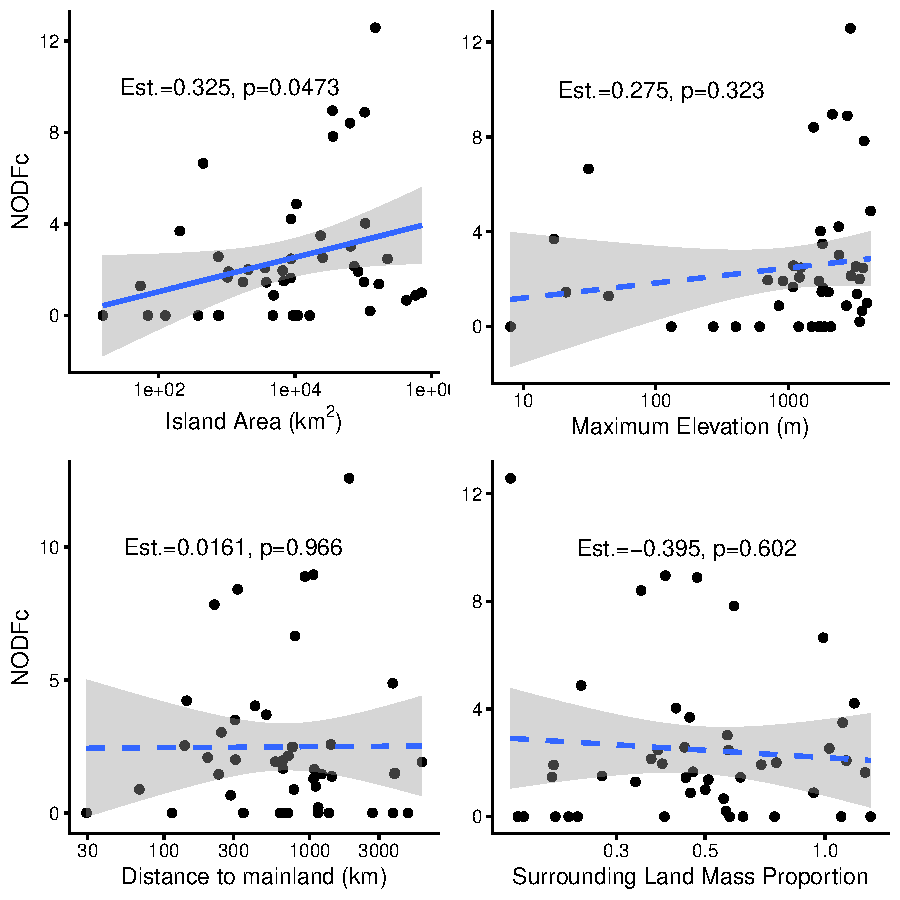
\includegraphics{HelmBiogeog/Figures/NODFc_plots.pdf}
    \caption{In addition to impacting network size, island area was positively related to $NODF_c$ such that larger islands were tended to be more nested on average (top left). In contrast, neither island elevation (top right) nor measures of island isolation including distance from the mainland (bottom left) or SLMP (bottom right) were significantly related to interaction nestedness within island networks.} %GF: Still need to add labels as well as fix cut off island area x-axis
    \label{fig:networkBG}
  \end{center}
\end{figure}

\clearpage


\begin{figure}[h!]
  \begin{center}
    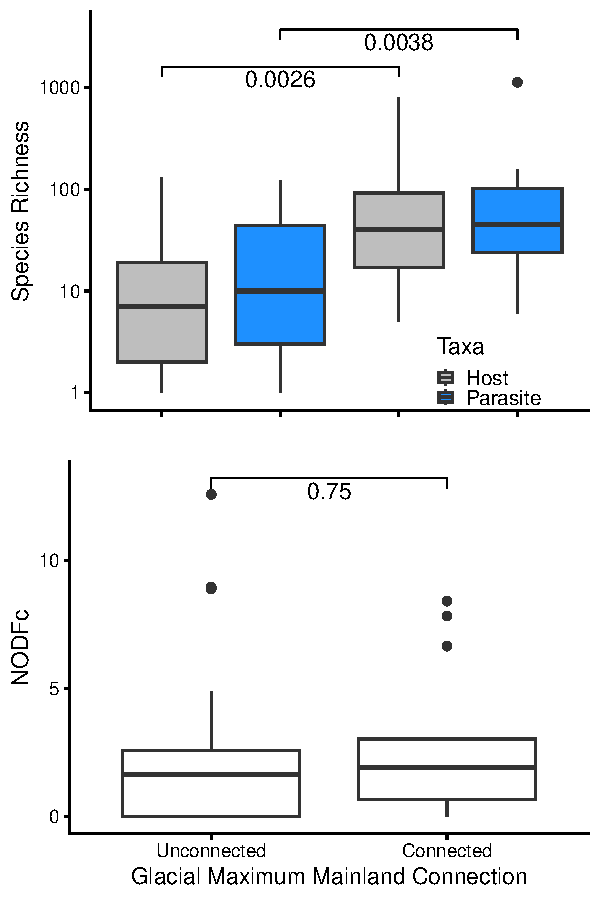
\includegraphics{HelmBiogeog/Figures/GMCC_NODFc_boxplots.pdf}
    \caption{Islands with a terrestrial connection to the mainland during the most recent glacial maximum have significantly higher host and helminth parasite diversity (top), but exhibit no significant differences in network nestedness. Comparison labels indicate p-values from a pairwise Wilcoxon test.}
    \label{fig:GMMC}
  \end{center}
\end{figure}













%--- Supplement ---

\clearpage

\section*{Supplemental Material}

\title{Island biogeography of host-helminth interaction networks}

\author[a,*]{Grant Foster}
\author[a,b]{Tad A Dallas}
% TAD: I don't think this will actually work, so maybe just write it out instead of trying to format it like main text. 

\affil[a]{Department of Biological Sciences, University of South Carolina, SC 29208, USA}
\affil[b]{Center for the Ecology of Infectious Diseases, University of Georgia, Athens, GA, 30602}


\renewcommand\Authands{ and }
\date{ \small *Corresponding author: grant.t.foster500@gmail.com}



\beginsupplement



\subsubsection*{The relationship between network size and nestedness}

Disentangling species richness (the sum of host and parasite richness) from nestedness is difficult, and many nestedness measures scale with species richness (Figure \ref{fig:richnessEffect}). Comparisons of properties across networks of different sizes is a non-trivial problem, and one potential solution is the implementation of a null modeling approach. In our case, we repeatedly shuffle links between hosts and helminths in each network, while maintaining both parasite host range (i.e., the number of host species a given parasite infects), and parasite species richness (i.e., the number of parasite species a host is infected by). For each network, we produced 1000 randomized networks, creating a distribution of spectral radii. Using these null distributions, we calculated $z$-scores, which measure the degree of divergence of the empirical network from the randomized null networks. Below, we present the correlations between alternative measures of network nestedness ($\eta$\citep{jonhson2013factors}, spectral radius, NODF, and $NODF_c$) as well as z-transformed versions of NODF and spectral radius. Nestedness as measured by $\eta$ was not standardized, as null model randomization for this measure is difficult, as randomized networks maintaining aspects of the degree distribution of host and parasite species will result in the same $\eta$ value as the empirical network. 

We find a significant correlation between the log-scale number of species within a network and all of the most common measures of network nestedness. However, as shown by \citet{song2017some}, $NODF_c$ is unrelated to network size or connectance across large sets of randomly generated networks. The relationship we observe across island networks may therefore reflect covariance with island area rather than a direct effect of network size on nestedness. Island area is positively associated with both network size \ref{fig:islandBG} and network nestedness \ref{fig:nestMod}, suggesting that area may act as a shared underlying driver that confounds the apparent association between network size and nestedness. As such, using metric sensitive to network size may give conflicting results. \ref{fig:Spectral.z_Results} illustrates that when using z-standardized NODF as our measure of interaction nestedness, we see the opposite relationship between island area and nestedness as with our $NODF_c$ metric, as well as relationships with elevational range and SLMP. In contrast, measuring interaction nestedness by the z-standardized spectral radius of a given graph yields qualitatively similar results to $NODF_c$ \ref{fig:Spectral.z_Results}.  

\begin{figure}[h!]
  \begin{center}
    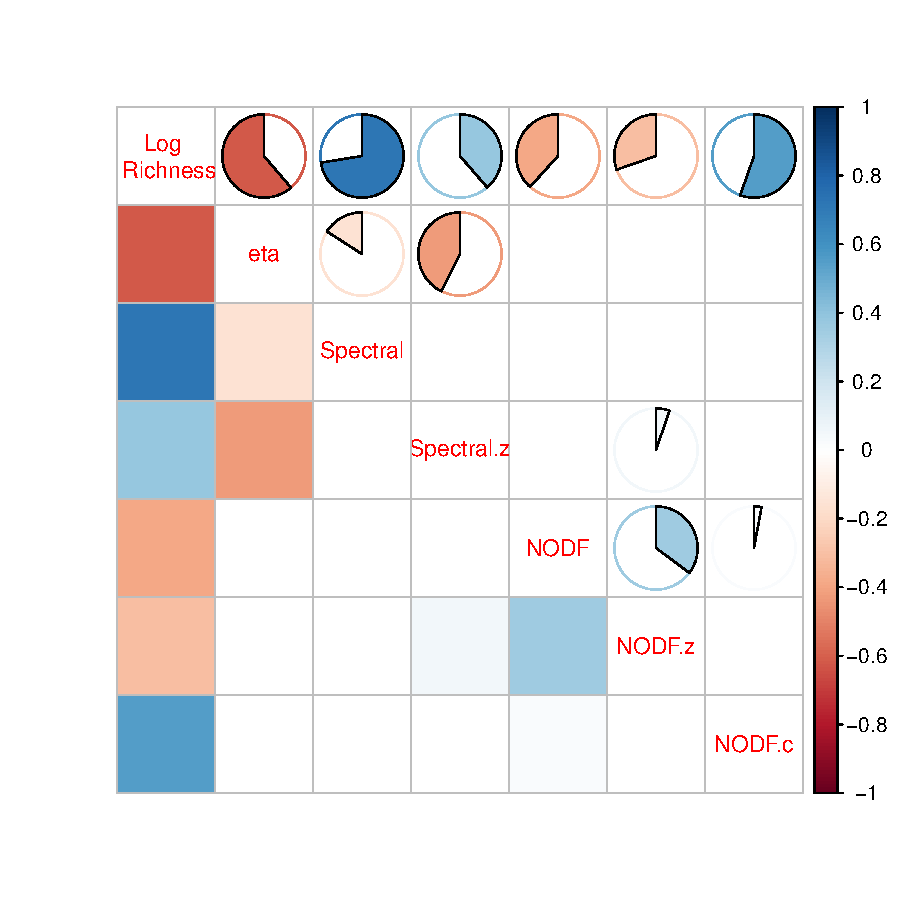
\includegraphics[width=\textwidth]{HelmBiogeog/Figures/Netsize_corplot.pdf}
    \caption{Correlogram visualizing Pearson's correlation coefficients between network size (log species richness) and alternative measures of network nestedness in our data. Shaded squares represent significant correlations (p-value $<0.05$). All measures of nestedness ($\eta$\citep{jonhson2013factors}, spectral radius, and NODF, as well as z-scores of the latter two based on null randomizations) are significantly correlated with network size in our dataset}
    \label{fig:richnessEffect}
  \end{center}
\end{figure}


\begin{figure}[h!]
  \begin{center}
    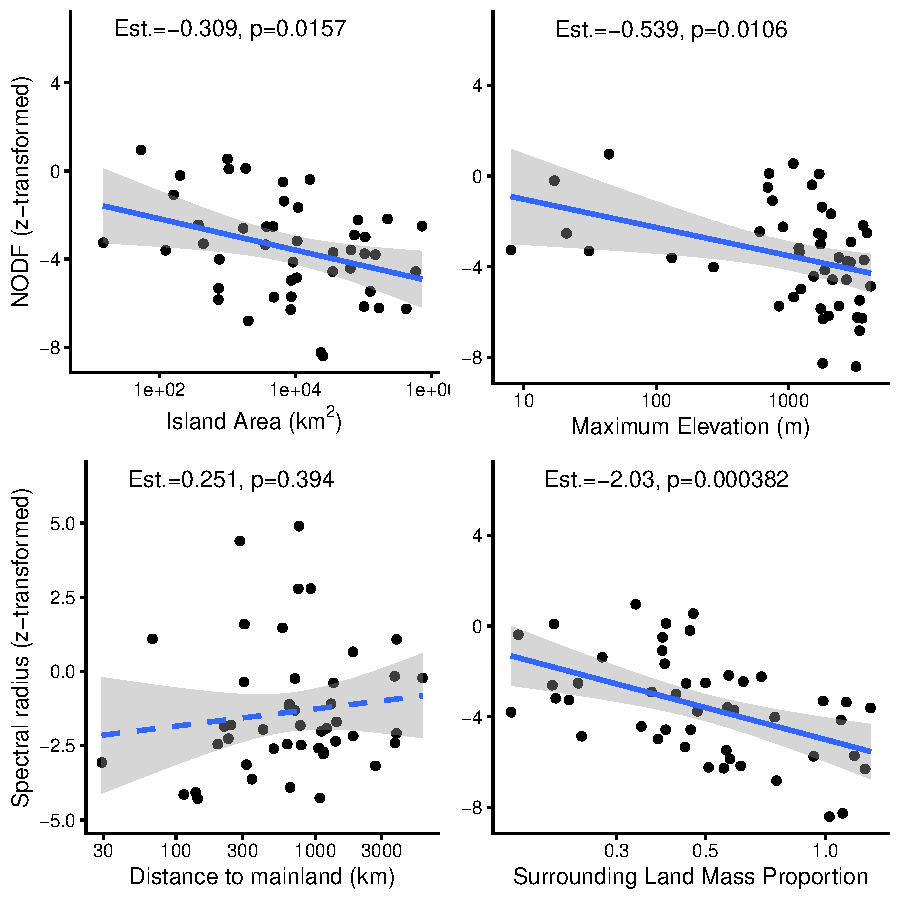
\includegraphics[width=\textwidth]{HelmBiogeog/Figures/NODF.z_Plots_Supplement.pdf}
    \caption{Recreation of Figure \ref{fig:networkBG} of the main text using z-transformed NODF as our nestedness metric of comparison. Despite null modeling approaches, this metric may still be sensitive to network size, and this gives conflicting results to those observed in $NODF_c$. }
    \label{fig:NODF.z_Results}
  \end{center}
\end{figure}

\clearpage

\begin{figure}[h!]
  \begin{center}
    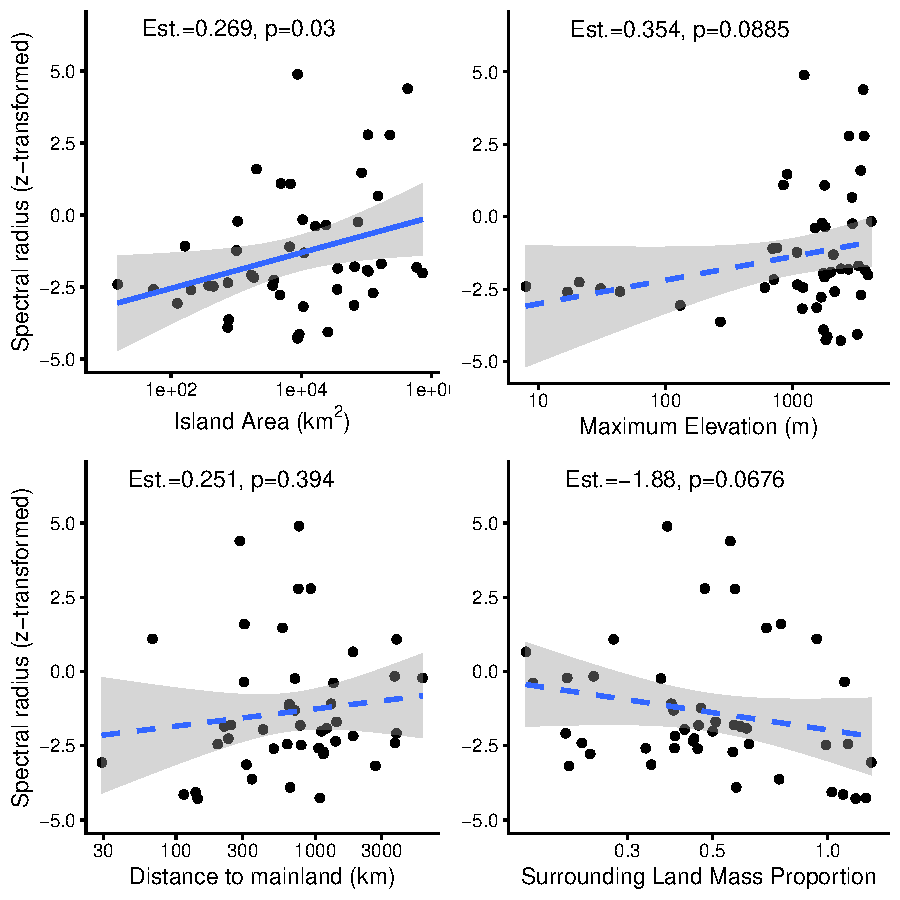
\includegraphics[width=\textwidth]{HelmBiogeog/Figures/Spectral.z_Plots_Supplement.pdf}
    \caption{Recreation of Figure \ref{fig:networkBG} of the main text using z-transformed spectral radius as our nestedness metric of comparison. In contrast to z-standardized NODF, spectral radius yields qualitatively similiar results to $NODF_c$ after z-transformation.}
    \label{fig:Spectral.z_Results}
  \end{center}
\end{figure}


\subsubsection*{Statistical Analysis}

In the main text, we use a negative binomial modeling multivariate regression approach to model the effects of island characteristics on species diversity. This approach greatly minimizes residual deviance compared to both Poisson and Quasi-Poisson GLMs \ref{tab:host_div_deviance}. Models incorporating island area and isolation as measured by SLMP yielded lowest AIC values, and as such are presented in the main text. 

\begin{table}[ht]
\centering
\caption{Model deviance diagnostics for host diversity models.}
\label{tab:host_div_deviance}
\begin{tabular}{lrrrr}
\hline
Model & Residual deviance & Residual df & AIC & Deviance/df \\
\hline
Poisson: Area + SLMP & 5621.91 & 55 & 5873.20 & 102.22 \\
Quasi-Poisson: Area + SLMP & 3497.06 & 55 & -- & 63.58 \\
Negative binomial: Area + Distance & 65.10 & 55 & 488.86 & 1.18 \\
Negative binomial: Area + SLMP & 63.90 & 55 & 481.30 & 1.16 \\
Negative binomial: Elevation + Distance & 69.24 & 55 & 515.87 & 1.26 \\
Negative binomial: Elevation + SLMP & 68.08 & 55 & 509.48 & 1.24 \\
\hline
\end{tabular}
\end{table}


Below, we report model diagnostic plots for the three models in the main text which show significant relationships between island characteristics and network properties. 

\begin{figure}[h!]
  \begin{center}
    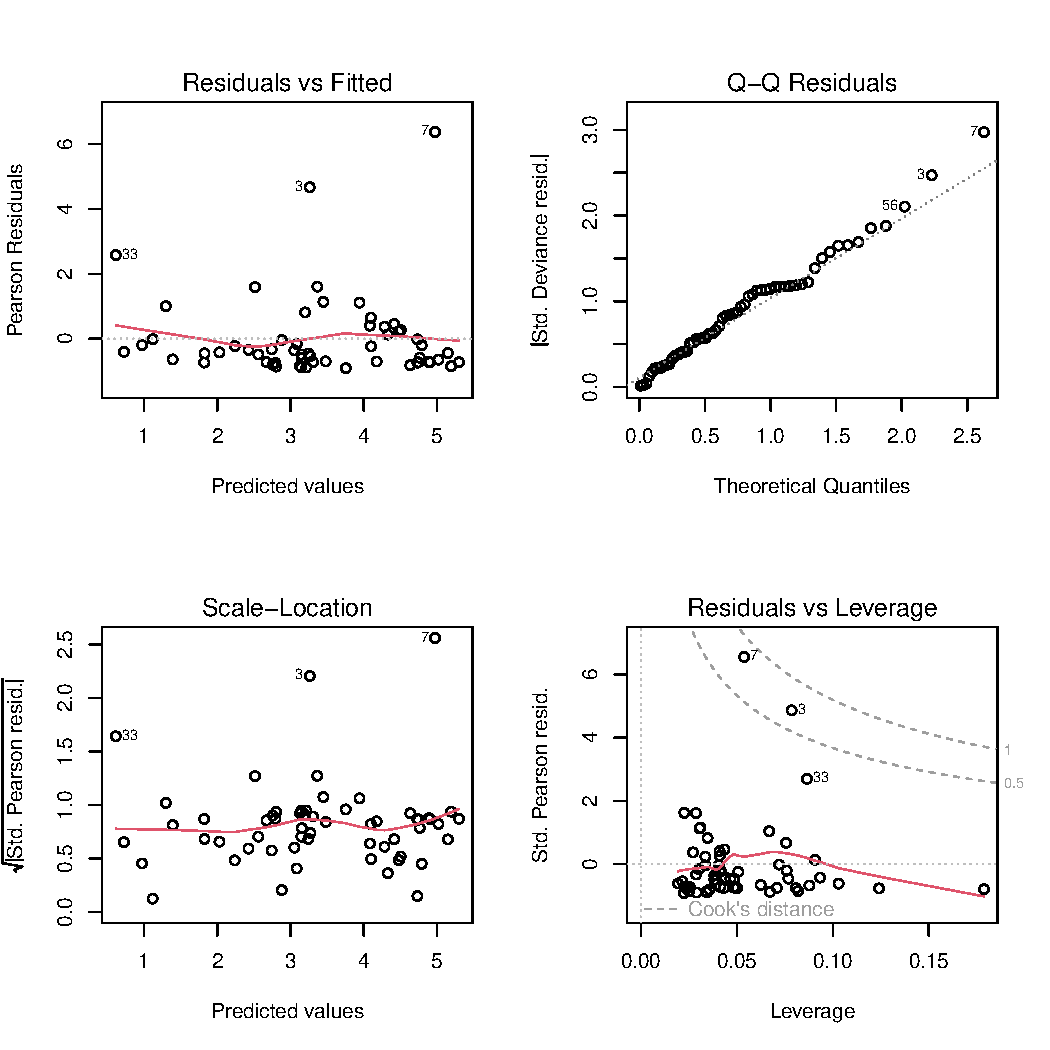
\includegraphics[width=\textwidth]{HelmBiogeog/Figures/ParDiv_diagnostics.pdf}
    \caption{Model diagnostics plots for our negative binomial model of \textbf{parasite richness} across islands, including residual vs fitted values (top left), Q-Q plot (top right), scale-location (bottom left), and residual vs leverage plot (bottom right), with dotted lines representing Cook's distance contours of 0.5 and 1, respectively. }
    \label{fig:parDivdiagnostics}
  \end{center}
\end{figure}

\begin{figure}[h!]
  \begin{center}
    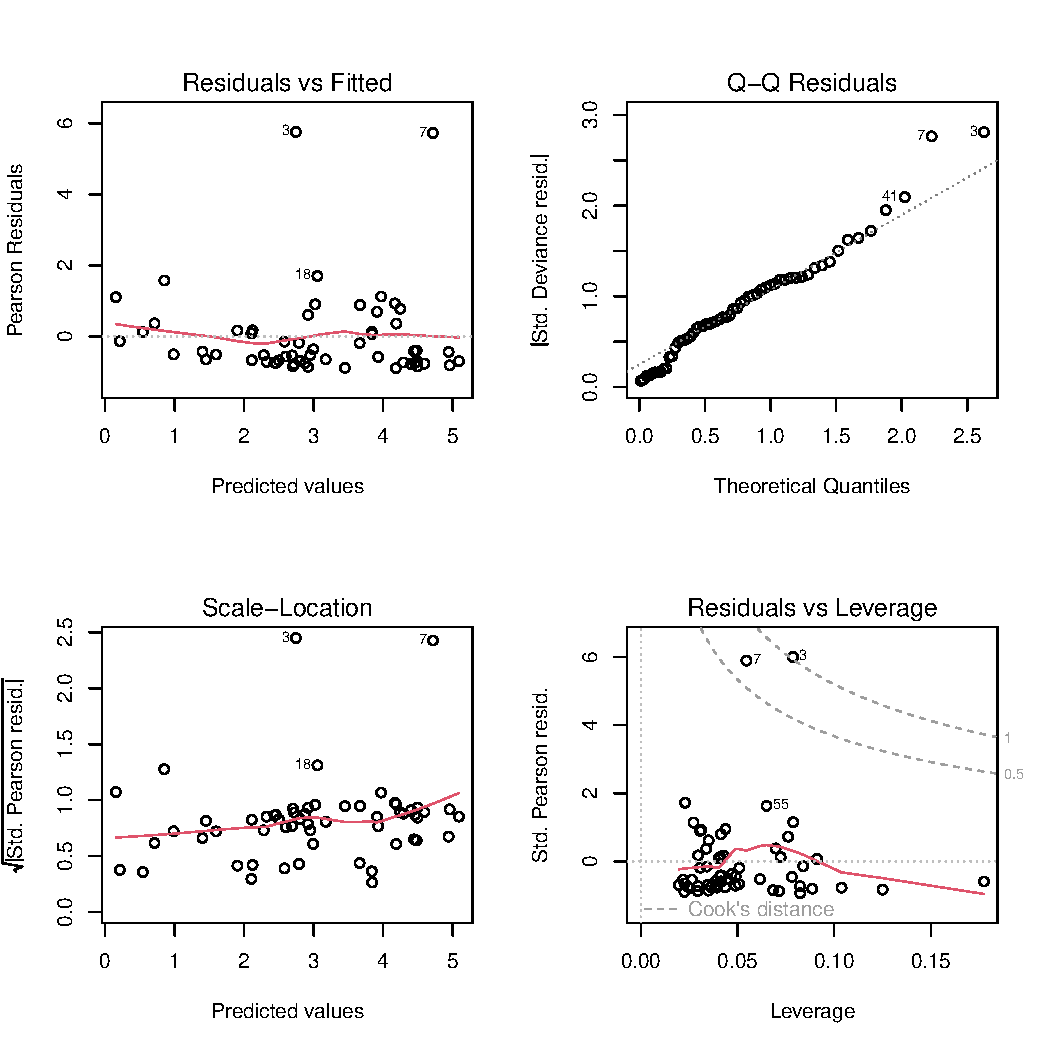
\includegraphics[width=\textwidth]{HelmBiogeog/Figures/HostDiv_diagnostics.pdf}
    \caption{Model diagnostics plots for our negative binomial model of \textbf{host richness} across islands, including residual vs fitted values (top left), Q-Q plot (top right), scale-location (bottom left), and residual vs leverage plot (bottom right), with dotted lines representing Cook's distance contours of 0.5 and 1, respectively. }
    \label{fig:hostDivdiagnostics}
  \end{center}
\end{figure}

\begin{figure}[h!]
  \begin{center}
    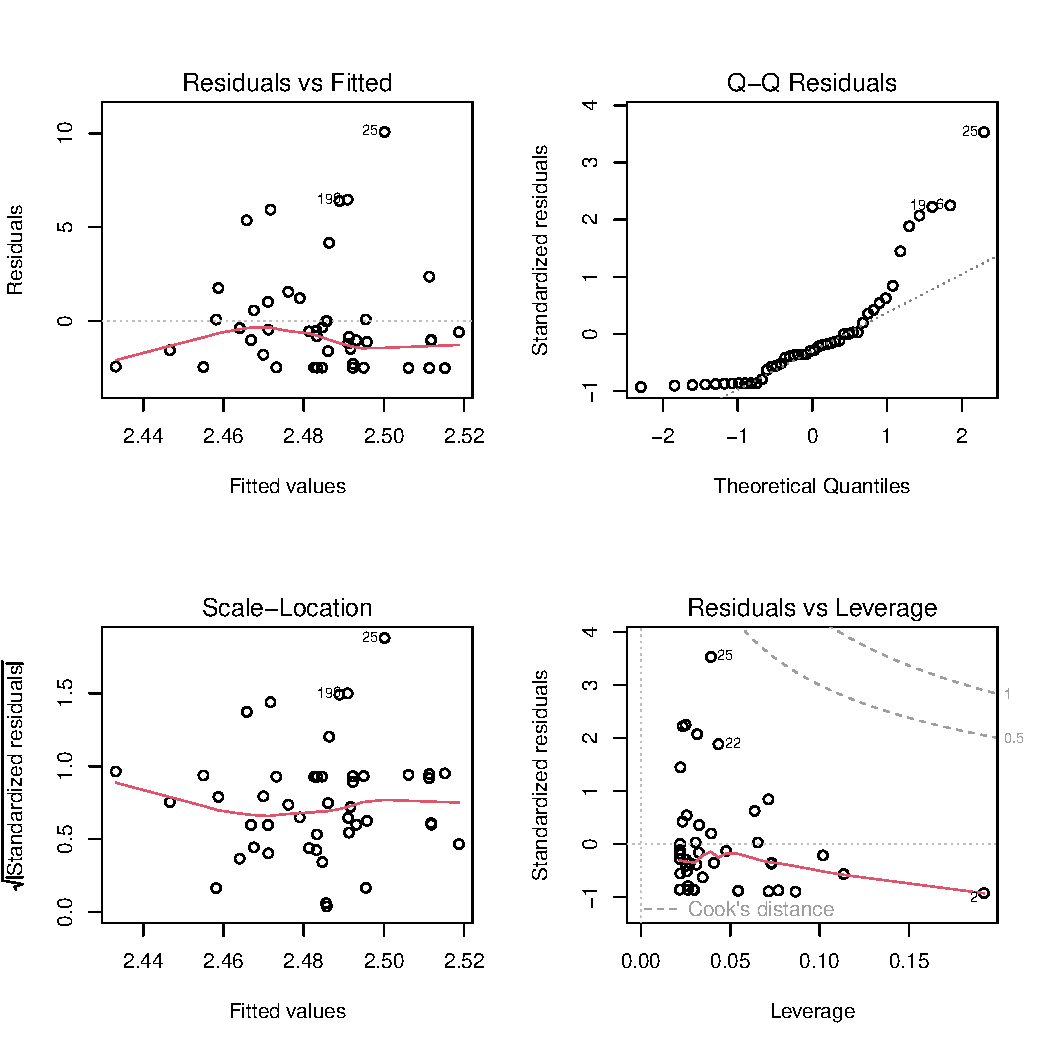
\includegraphics[width=\textwidth]{HelmBiogeog/Figures/NODFc_Distance_diagnostics.pdf}
    \caption{Model diagnostics plots for our generalized linear model of \textbf{network nestedness ($NODF_c$)} across islands, including residual vs fitted values (top left), Q-Q plot (top right), scale-location (bottom left), and residual vs leverage plot (bottom right), with dotted lines representing Cook's distance contours of 0.5 and 1, respectively. }
    \label{fig:nodfcdiagnostics}
  \end{center}
\end{figure}

\clearpage\\

\subsubsection*{The relationship between nestedness and modularity}

We don't consider modularity in the main text, but we explore it here for fun, as it is closely related to nestedness. Cite arxiv paper and Fortuna 2010 \citep{fortuna2010nestedness} and say that they are like...the same thing.


GF: How necessary do you think this addition is? Can add it back in if you think so, but would need to recalculate on our new network sets. 
\clearpage
